\section{Introduction}
	
	\subsection{Système d'exploitation}
		Un système d’exploitation (\textbf{SE} ou \textbf{OS} pour \textit{operating system}) est un ensemble de programmes qui dirigent l'utilisation des capacités d’un ordinateur par des logiciels applicatifs (applications ou programmes directement utilisés par l’utilisateur). Il reçoit des demandes d'utilisation des capacités de l'ordinateur (capacité de stockage des mémoires et des disques durs, capacité de calcul du processeur, capacités de communication vers des périphériques ou via le réseau) de la part des logiciels applicatifs. Le système d'exploitation accepte ou refuse ces demandes, puis réserve les ressources en question pour éviter que leur utilisation n'interfère avec d'autres demandes provenant d'autres logiciels.
		
		\paragraph{} Lorsqu'un programme désire accéder à une ressource matérielle, il ne lui est pas nécessaire d'envoyer des informations spécifiques au périphérique, il lui suffit d'envoyer les informations au système d'exploitation, qui se charge de les transmettre au périphérique concerné via son pilote. En l'absence de pilotes il faudrait que chaque programme reconnaisse et prenne en compte la communication avec chaque type de périphérique.
	
		\begin{center}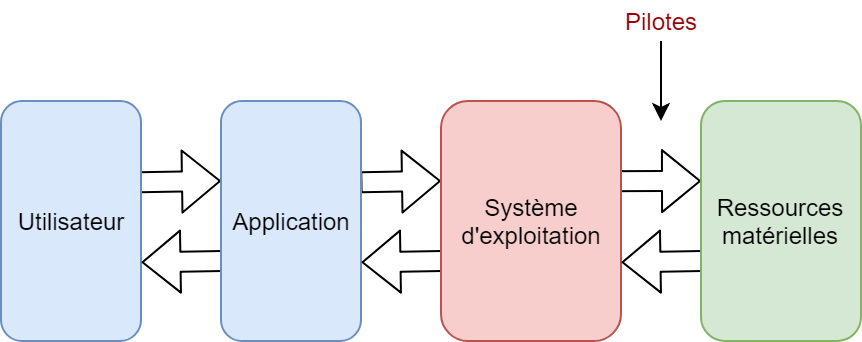
\includegraphics[scale=0.4]{../img/SE.png}\end{center}

		Le système d’exploitation est donc chargé d'assurer la liaison entre les ressources matérielles, l'utilisateur et les applications. Il permet ainsi de dissocier les programmes et le matériel, afin notamment d'assurer la \textbf{gestion des ressources} et offrir à l'utilisateur une interface homme-machine notée IHM simplifiée lui permettant de s'affranchir de la complexité de la machine physique.

		\subsubsection*{Rôles du système d'exploitation :}
			\begin{itemize}
				\item \textbf{\textit{Gestion du processeur }:} gère l'allocation du processeur entre les différents programmes avec un algorithme d'ordonnancement. Le type d'ordonnanceur est totalement dépendant du système d'exploitation, en fonction de l'objectif visé.
				\item \textbf{\textit{Gestion de la mémoire vive }:} gère l'espace mémoire alloué à chaque application et, le cas échéant, à chaque usager. En cas d'insuffisance de mémoire physique, le système d'exploitation peut créer une zone mémoire sur le disque dur, appelée mémoire virtuelle. La mémoire virtuelle permet de faire fonctionner des applications nécessitant plus de mémoire qu'il n'y a de mémoire vive disponible sur le système. En contrepartie cette mémoire est beaucoup plus lente.
				\item \textbf{\textit{Gestion des entrées/sorties }:} permet d'unifier et de contrôler l'accès des programmes aux ressources matérielles par l'intermédiaire des pilotes (appelés également gestionnaires de périphériques ou gestionnaires d'entrée/sortie).
				\item \textbf{\textit{Gestion de l'exécution des applications }:} chargé de la bonne exécution des applications en leur affectant les ressources nécessaires à leur bon fonctionnement. Il permet à ce titre de «tuer» une application ne répondant plus correctement.
				\item \textbf{\textit{Gestion des droits }:} chargé de la sécurité liée à l'exécution des programmes en garantissant que les ressources ne sont utilisées que par les programmes et utilisateurs possédant les droits adéquats.
				\item \textbf{\textit{Gestion des fichiers }:} le système d'exploitation gère la lecture et l'écriture dans le système de fichiers et les droits d'accès aux fichiers par les utilisateurs et les applications.
				\item \textbf{\textit{Gestion des informations }:} le système d'exploitation fournit un certain nombre d'indicateurs permettant de diagnostiquer le bon fonctionnement de la machine.
			\end{itemize}
		
		\subsubsection*{Composantes du système d'exploitation :}
			Le système d'exploitation est composé d'un ensemble de logiciels permettant de gérer les interactions avec le matériel, parmi eux :
			\begin{itemize}
				\item \textbf{\textit{Le noyau (kernel) }:} représentant les fonctions fondamentales du système d'exploitation telles que la gestion de la mémoire, des processus, des fichiers, des entrées-sorties principales, et des fonctionnalités de communication.
				\item \textbf{\textit{L'interpréteur de commande (shell, traduisez "coquille" par opposition au noyau) }:} permettant la communication avec le système d'exploitation par l'intermédiaire d'un langage de commandes, afin de permettre à l'utilisateur de piloter les périphériques en ignorant tout des caractéristiques du matériel qu'il utilise, de la gestion des adresses physiques, etc.
				\item \textbf{\textit{Le système de fichiers (en anglais «file system», noté FS) }:} permettant d'enregistrer les fichiers dans une arborescence.
			\end{itemize}
		
		\subsubsection*{Amorcage :}
			Le système d'exploitation est le premier programme exécuté lors de la mise en marche de l'ordinateur, après l’amorçage. L’amorçage ou le boot (\textit{to pull oneself up by one’s bootstrap}) est la procédure de démarrage d’un ordinateur qui comporte notamment le chargement du programme initial (le système d'exploitation).\\
			Le problème posé par le boot est de faire démarrer un ordinateur et lui faire charger un programme alors que, a priori, il ne possède encore aucun programme dans sa mémoire. L’ordinateur exploite en fait un programme réduit, le chargeur d'amorçage, permettant d’extraire un programme accessible via un périphérique de stockage permanent ou amovible. Ce dernier est typiquement le \textbf{noyau du système d’exploitation}, qui s’installera en RAM et appellera lui-même des programmes applicatifs.
			On distingue :
			\begin{itemize}
				\item le démarrage à froid (\textit{cold boot}) : allumer une machine éteinte
				\item le démarrage à chaud (\textit{warm boot} ou \textit{reboot}) : recharger le programme initial (sans coupure de l’alimentation électrique)
			\end{itemize}
			Au démarrage de l’ordinateur, la première chose qui s'affiche à l'écran est l'écran de boot. Cet écran varie beaucoup selon les ordinateurs parce qu'il dépend du matériel dont est constituée la machine. C'est en effet la carte mère qui affiche l'écran de boot. La carte mère est le composant fondamental de tout ordinateur, puisque c'est elle qui fait fonctionner le processeur, les disques durs, le lecteur de CD-ROM, etc. Ensuite, le système d’exploitation se lance. C'est seulement une fois qu’il est chargé que l’on peut utiliser les programmes.
	
	
	\subsection{Programmation système}
		La \textit{\textbf{programmation système}} est un type de programmation qui vise au développement de programmes qui font partie du système d’exploitation d’un ordinateur ou qui en réalisent les fonctions. Elle se distingue de la \textit{\textbf{programmation des applications}} en ce qu’elle s’intéresse non pas au traitement des données, mais à la résolution des problèmes pour les humains, aux interfaces (API), aux protocoles (communication) et à la gestion des ressources.\\
		En réalité, seuls les \textit{\textbf{programmes d'application}} sont utilisés pas les utilisateurs. Les \textit{\textbf{programmes système}} le sont implicitement. La programmation système inclut, en outre, l’accès aux fichiers, la gestion de la mémoire vive et des processeurs et la programmation de tous les périphériques qui font entrer ou sortir de l’information d’un ordinateur (clavier, écran, modems...). Elle permet donc de communiquer avec ces périphériques, créer des pilotes, voire même créer un système d'exploitation.
		
		\subsubsection*{Programmation système en C sous UNIX :} 
			La programmation système se fait généralement par le biais de langages tel que le langage \textit{\textbf{assembleur}}, et d’un langage de bas niveau. C’est le cas des systèmes d’exploitation de type \textbf{UNIX} (Linux, FreeBSD, Solaris…) dont 90\% du code est écrit en \textit{\textbf{langage C}} (qui a été spécialement créé pour le développement du système UNIX), le reste est écrit en assembleur suivant les architectures cibles (x86, SPARC...).
			
			\paragraph{} Les systèmes UNIX sont des systèmes d'exploitation qui sont constitués de plusieurs programmes, et chacun d'eux fournit un service au système. Tous les programmes qui fournissent des services similaires sont regroupés dans une \textit{\textbf{couche logicielle}}. Une couche logicielle qui a accès au matériel informatique s'appelle une \textit{\textbf{couche d'abstraction matérielle}}. Le \textit{\textbf{noyau}} est une sorte de logiciel d'arrière-plan qui assure les communications entre ces programmes. C'est donc par lui qu'il va falloir passer pour avoir accès aux informations du système.
			
			\paragraph{} Pour accéder à ces informations du système, on utilise des fonctions qui permettent de communiquer avec le noyau. Ces fonctions s'appellent des \textit{\textbf{appels-systèmes}}. Le terme \textit{\textbf{appel-système}} désigne l'appel d'une fonction, qui, depuis l'espace utilisateur, demande des services ou des ressources au système d'exploitation.\\
			Chaque architecture matérielle ne supporte que sa propre liste d'appels-systèmes, c'est pourquoi les appels-systèmes diffèrent d'une machine à l'autre. Mais la plupart d'entre eux sont implémentés sur toutes les machines.

			\paragraph{} Pour des raisons de sécurité évidentes, les applications de l'espace utilisateur ne peuvent pas directement exécuter le code du noyau ou manipuler ses données. Par conséquent, un mécanisme de signaux a été mis en place. Quand une application exécute un appel-système, elle peut alors effectuer un \textit{\textbf{trap}} (permutation de l'exécution de l'application en mode noyau), et peut exécuter le code, du moment que le noyau le lui autorise.
